\subsection{Caso de Prueba 3 — \textit{Kicked Kepler}}

El experimento “Kicked Kepler” analiza un sistema Kepleriano perturbado: una estrella central y un planeta ligero sometidos a impulsos periódicos en su velocidad orbital. El caso busca ajustar las masas dentro de rangos restringidos para reducir la respuesta caótica del sistema, medida mediante el exponente de Lyapunov, al tiempo que preserva la periodicidad inducida por los impulsos.

\paragraph{A. Propósito}
Cuantificar cómo el pipeline híbrido (GA + refinamiento continuo) puede estabilizar una órbita Kepleriana sujeta a impulsos periódicos. Se contrasta el comportamiento del estado base con el de la solución óptima reportada por el notebook, considerando tanto el exponente de Lyapunov como la penalización de periodicidad aplicada tras cada ciclo de impulsos.

\paragraph{B. Parámetros críticos del experimento}
El diccionario \texttt{case} captura los horizontes de integración, condiciones iniciales y configuración del controlador. Se trabaja en unidades astronómicas (UA), años y masas solares.

\begin{listing}[H]
\caption{Declaración del diccionario \texttt{case} en el notebook Caso03}
\label{lst:c03_case} %chktex 24
\begin{adjustbox}{max width=\textwidth}
\begin{minipage}{\textwidth}
\begin{minted}[fontsize=\small, breaklines, breakanywhere]{python}
case = {
    # Integración (UA, años, masas solares)
    "t_end_short": 0.5,
    "t_end_long": 4.0,
    "dt": 2.0e-4,
    "integrator": "ias15",

    # Estado inicial (estrella + planeta tipo Tierra)
    "r0": ((0.0, 0.0, 0.0), (1.0, 0.0, 0.0)),
    "v0": ((0.0, 0.0, 0.0), (0.0, 6.2831853072, 0.0)),

    # Rangos de masa
    "mass_bounds": ((0.8, 1.2), (2.8e-6, 3.4e-2)),

    # Parámetros de los impulsos (“kicks”)
    "kick_period": 0.25,
    "kick_delta_v": 0.05,

    # Penalización de periodicidad
    "periodicity_weight": 0.25,

    # Algoritmo genético
    "pop_size": 160,
    "n_gen_step": 5,
    "crossover": 0.9,
    "mutation": 0.2,
    "elitism": 2,
    "seed": 2024,

    # Optimización continua
    "max_epochs": 45,
    "top_k_long": 10,
    "stagnation_window": 5,
    "stagnation_tol": 1.0e-4,
    "local_radius": 0.05,
    "radius_decay": 0.88,
    "time_budget_s": 1800.0,
    "eval_budget": 14000,

    # Artefactos / modo gráfico
    "artifacts_dir": "artifacts/kicked_kepler",
    "save_plots": True,
    "headless": False,
}
\end{minted}
\end{minipage}
\end{adjustbox}
\end{listing}

\begin{table}[H]
\centering
\caption{Resumen de parámetros críticos del Caso 03}
\label{tab:c03_params} %chktex 24
\begin{tabularx}{\textwidth}{@{}l>{\raggedright\arraybackslash}X@{}}
\toprule
\textbf{Componente} & \textbf{Descripción} \\
\midrule
Horizontes y paso & $t_{\text{short}} = 0.5$ años, $t_{\text{long}} = 4.0$ años, paso $\Delta t = 2\times 10^{-4}$ años con integrador \texttt{IAS15}. \\
Estado inicial & Estrella en reposo, planeta en $(1,0,0)$ UA con velocidad circular $(0,2\pi,0)$ UA/año. \\
Rangos de masa & Estrella $[0.8,1.2]$ M$_\odot$, planeta $[2.8\times10^{-6},3.4\times10^{-2}]$ M$_\odot$. \\
Impulsos & Periodo de “kick” $0.25$ años, incremento de velocidad tangencial $0.05$ UA/año. \\
Penalización & \texttt{periodicity\_weight} $=0.25$ incentiva la repetición del estado tras cada ciclo de impulsos. \\
GA & Población 160, cruce 0.9, mutación 0.2, elitismo 2, semilla 2024, $top\_k\_long = 10$. \\
Optimización continua & 45 épocas máximo, radio local 0.05 con decaimiento 0.88, tolerancia $10^{-4}$. \\
Artefactos & Resultados en \texttt{artifacts/kicked\_kepler}, modo gráfico activo (\texttt{headless} = False). \\
\bottomrule
\end{tabularx}
\end{table}

\paragraph{C. Desglose detallado de celdas de código}
Se describe cada celda de código relevante, incluyendo el fragmento ejecutado y la salida esperada. Las celdas de markdown proporcionan el hilo conductor narrativo.

\subsubsection*{Celda 3 — Preparación de rutas}
\paragraph{Descripción} Localiza la raíz del repositorio \texttt{two\_body}, la añade a \texttt{sys.path} y detiene la ejecución si no la encuentra.
\paragraph{Código}
\par\smallskip
\begin{listing}[H]
\caption{Celda 3: detección de la raíz del proyecto}
\begin{adjustbox}{max width=\textwidth}
\begin{minipage}{\textwidth}
\begin{minted}[fontsize=\small, breaklines, breakanywhere]{python}
import sys
from pathlib import Path
PROJECT_ROOT = Path.cwd().resolve()
while PROJECT_ROOT.name != 'two_body' and PROJECT_ROOT.parent != PROJECT_ROOT:
    PROJECT_ROOT = PROJECT_ROOT.parent
if PROJECT_ROOT.name != 'two_body':
    raise RuntimeError('No se encontró la carpeta two_body')
PARENT = PROJECT_ROOT.parent
if str(PARENT) not in sys.path:
    sys.path.insert(0, str(PARENT))
print('PYTHONPATH += ', PARENT)
\end{minted}
\end{minipage}
\end{adjustbox}
\end{listing}
\paragraph{Salida esperada} Mensaje tipo \texttt{PYTHONPATH += /ruta/al/directorio/padre}.

\subsubsection*{Celda 5 — Importaciones principales}
\paragraph{Descripción} Importa configuraciones, controlador, visualizadores y Rebound, junto con NumPy.
\paragraph{Código}
\par\smallskip
\begin{listing}[H]
\caption{Celda 5: importación de componentes}
\begin{adjustbox}{max width=\textwidth}
\begin{minipage}{\textwidth}
\begin{minted}[fontsize=\small, breaklines, breakanywhere]{python}
from two_body import Config, set_global_seeds
from two_body.core.telemetry import setup_logger
from two_body.logic.controller import ContinuousOptimizationController
from two_body.presentation.visualization import Visualizer as PlanarVisualizer
from two_body.presentation.triDTry import Visualizer as Visualizer3D
from two_body.simulation.rebound_adapter import ReboundSim
import numpy as np
from pathlib import Path
\end{minted}
\end{minipage}
\end{adjustbox}
\end{listing}
\paragraph{Salida esperada} Sin salida; cualquier excepción delataría dependencias faltantes.

\subsubsection*{Celda 7 — Instrumentación de timings}
\paragraph{Descripción} Activa \texttt{PERF\_TIMINGS\_ENABLED} y carga utilidades para manipular los CSV de tiempos.
\paragraph{Código}
\par\smallskip
\begin{listing}[H]
\caption{Celda 7: configuración de \texttt{perf\_timings}}
\begin{adjustbox}{max width=\textwidth}
\begin{minipage}{\textwidth}
\begin{minted}[fontsize=\small, breaklines, breakanywhere]{python}
import os
os.environ['PERF_TIMINGS_ENABLED'] = '1'
os.environ.setdefault('PERF_TIMINGS_JSONL', '0')
from two_body.perf_timings.timers import time_block
from two_body.perf_timings import latest_timing_csv, read_timings_csv, parse_sections_arg, filter_rows
\end{minted}
\end{minipage}
\end{adjustbox}
\end{listing}
\paragraph{Salida esperada} Sin salida.

\subsubsection*{Celda 9 — Handler de logging para Jupyter}
\paragraph{Descripción} Define un \texttt{logging.Handler} personalizado para mostrar los mensajes del controlador en la celda.
\paragraph{Código}
\par\smallskip
\begin{listing}[H]
\caption{Celda 9: configuración de logs interactivos}
\begin{adjustbox}{max width=\textwidth}
\begin{minipage}{\textwidth}
\begin{minted}[fontsize=\small, breaklines, breakanywhere]{python}
import logging
from IPython.display import display, Markdown

class NotebookHandler(logging.Handler):

    def __init__(self):
        super().__init__()
        self.lines = []

    def emit(self, record):
        msg = self.format(record)
        self.lines.append(msg)
        print(msg)
handler = NotebookHandler()
handler.setFormatter(logging.Formatter('[%(asctime)s] %(levelname)s - %(message)s'))
logger = setup_logger(level='INFO')
logger.handlers.clear()
logger.addHandler(handler)
logger.setLevel(logging.INFO)
\end{minted}
\end{minipage}
\end{adjustbox}
\end{listing}
\paragraph{Salida esperada} Sin salida inmediata; los logs de optimización se verán más adelante.

\subsubsection*{Celda 11 — Declaración del escenario}
\paragraph{Descripción} Define el diccionario \texttt{case}; véase Listing~\ref{lst:c03_case}.
\paragraph{Salida esperada} Sin salida.

\subsubsection*{Celda 12 — Instanciación de \texttt{Config}}
\paragraph{Descripción} Construye \texttt{cfg = Config(**case)} y obtiene un logger base. % chktex 36
\paragraph{Código}
\begin{listing}[H]
\caption{Celda 12: creación de la configuración de trabajo}
\par\smallskip
\begin{adjustbox}{max width=\textwidth}
\begin{minipage}{\textwidth}
\begin{minted}[fontsize=\small, breaklines, breakanywhere]{python}
from two_body.logic.controller import ContinuousOptimizationController
from two_body.core.config import Config
from two_body.core.telemetry import setup_logger
from two_body.core.cache import HierarchicalCache
cfg = Config(**case)
logger = setup_logger()
\end{minted}
\end{minipage}
\end{adjustbox}
\end{listing}
\paragraph{Salida esperada} Sin salida.

\subsubsection*{Celda 14 — Ajuste del adaptador REBOUND (impulsos)}
\paragraph{Descripción} Define una subclase de \texttt{ReboundSim} que aplica los impulsos periódicos en la partícula ligera y reasigna \texttt{ReboundSim} en el módulo de simulación.
\paragraph{Código}
\par\smallskip
\begin{listing}[H]
\caption{Celda 14: monkeypatch del adaptador con “kicks” \texttt{kick\_periodic}}
\begin{adjustbox}{max width=\textwidth}
\begin{minipage}{\textwidth}
\begin{minted}[fontsize=\small, breaklines, breakanywhere]{python}
class KickReboundSim(ReboundSim):

    def setup_simulation(self, masses, r0, v0, **kwargs):
        sim = super().setup_simulation(masses, r0, v0, **kwargs)
        kick_period = case.get('kick_period', 0.25)
        kick_delta_v = case.get('kick_delta_v', 0.05)

        def kick(sim_ptr):
            t = sim.t
            if abs(t / kick_period - round(t / kick_period)) < 0.001:
                if len(sim.particles) > 1:
                    body = sim.particles[1]
                    body.vy += kick_delta_v
        sim.post_timestep_modifications = kick
        return sim
from two_body.simulation import rebound_adapter
rebound_adapter.ReboundSim = KickReboundSim
\end{minted}
\end{minipage}
\end{adjustbox}
\end{listing}
\paragraph{Salida esperada} Sin salida; a partir de esta celda toda simulación REBOUND inyectará los impulsos definidos.

\subsubsection*{Celda 15 — Chequeo de hiperparámetros}
\paragraph{Descripción} Imprime los rangos de massa, máximo de épocas y presupuesto de evaluaciones.
\paragraph{Código}
\par\smallskip
\begin{listing}[H]
\caption{Celda 15: verificación rápida}
\begin{adjustbox}{max width=\textwidth}
\begin{minipage}{\textwidth}
\begin{minted}[fontsize=\small, breaklines, breakanywhere]{python}
print(cfg.mass_bounds, cfg.max_epochs, cfg.eval_budget)
\end{minted}
\end{minipage}
\end{adjustbox}
\end{listing}
\paragraph{Salida esperada} Línea con los valores impresos.

\begin{listing}[H]
\caption{Ejemplo Salida}
\begin{adjustbox}{max width=0.7\textwidth}
\begin{minipage}{\textwidth}
\begin{minted}[fontsize=\small, breaklines, breakanywhere]{bash}
((0.8, 1.2), (2.8e-06, 0.034)) 50 16000
\end{minted}
\end{minipage}
\end{adjustbox}
\end{listing}

\subsubsection*{Celda 17 — Ejecución del controlador}
\paragraph{Descripción} Lanza el controlador evolutivo dentro de \texttt{time\_block(``notebook\_run'')}; los logs de cada época aparecen en la celda. % chktex 36
\paragraph{Código}
\par\smallskip
\begin{listing}[H]
\caption{Celda 17: lanzamiento de la optimización}
\begin{adjustbox}{max width=\textwidth}
\begin{minipage}{\textwidth}
\begin{minted}[fontsize=\small, breaklines, breakanywhere]{python}
with time_block('notebook_run', extra={'source': 'Caso03.ipynb'}):
    controller = ContinuousOptimizationController(cfg, logger=logger)
    results = controller.run()
\end{minted}
\end{minipage}
\end{adjustbox}
\end{listing}
\paragraph{Salida esperada} Serie de logs por época y registro del tiempo total del bloque \texttt{notebook\_run}.

\begin{listing}[H]
\caption{Ejemplo Salida}
\begin{adjustbox}{max width=0.7\textwidth}
\begin{minipage}{\textwidth}
\begin{minted}[fontsize=\small, breaklines, breakanywhere]{bash}
[2025-11-02 18:03:24,171] INFO - Starting optimization | pop=180 | dims=2 | time_budget=1800.0s | eval_budget=16000
[2025-11-02 18:03:34,260] INFO - Epoch 0 | new global best (short) lambda=-0.608653 | fitness=-0.130490 | penalty=14.782862 | masses=(1.076408, 0.009538)
[2025-11-02 18:03:39,255] INFO - Epoch 0 | new global best (long) lambda=0.078349 | fitness=-0.112894 | penalty=0.690898 | masses=(1.112924, 0.018475)
...
[2025-11-02 18:12:12,443] INFO - Epoch 32 | new global best (short) lambda=-2.569736 | fitness=1.825861 | penalty=14.877505 | masses=(1.045259, 3e-06)
[2025-11-02 18:12:18,320] INFO - Epoch 32 complete | lambda_short=-2.569736 | fitness_short=1.825861 | lambda_best=-2.569736 | fitness_best=1.825861 | evals short/long=180/12 | total evals=6336 | radius=0.0209
...
[2025-11-02 18:16:32,481] INFO - Stagnation detected; reseeding around best candidate.
[2025-11-02 18:16:32,481] INFO - Epoch 47 complete | lambda_short=-0.551856 | fitness_short=-0.191244 | lambda_best=-2.569736 | fitness_best=1.825861 | evals short/long=180/12 | total evals=9216 | radius=0.0128
[2025-11-02 18:16:49,298] INFO - Epoch 48 complete | lambda_short=-2.546347 | fitness_short=1.804238 | lambda_best=-2.569736 | fitness_best=1.825861 | evals short/long=180/12 | total evals=9408 | radius=0.0128
[2025-11-02 18:17:05,979] INFO - Epoch 49 complete | lambda_short=-0.266154 | fitness_short=-0.477131 | lambda_best=-2.569736 | fitness_best=1.825861 | evals short/long=180/12 | total evals=9600 | radius=0.0128
[2025-11-02 18:17:05,980] INFO - Optimization completed | epochs=50 | evals=9600 | best lambda=-2.569736 | wall=821.8s
\end{minted}
\end{minipage}
\end{adjustbox}
\end{listing}

\subsubsection*{Celda 19 — Métricas y resultados}
\paragraph{Descripción} Captura \texttt{metrics} y muestra \texttt{results} para inspeccionar la mejor solución encontrada.
\paragraph{Código}
\par\smallskip
\begin{listing}[H]
\caption{Celda 19: inspección de resultados}
\begin{adjustbox}{max width=\textwidth}
\begin{minipage}{\textwidth}
\begin{minted}[fontsize=\small, breaklines, breakanywhere]{python}
metrics = controller.metrics
results
\end{minted}
\end{minipage}
\end{adjustbox}
\end{listing}
\paragraph{Salida esperada} Diccionario con \texttt{status}, \texttt{best}, \texttt{evals}, \texttt{epochs}; los valores dependen de la corrida.

\begin{listing}[H]
\caption{Ejemplo Salida}
\begin{adjustbox}{max width=0.7\textwidth}
\begin{minipage}{\textwidth}
\begin{minted}[fontsize=\small, breaklines, breakanywhere]{bash}
{'status': 'completed',
 'best': {'masses': [1.045258635678602, 2.8e-06],
  'lambda': -2.569736031111161,
  'fitness': 1.825860801467893,
  'm1': 1.045258635678602,
  'm2': 2.8e-06},
 'evals': 9600,
 'epochs': 50}
\end{minted}
\end{minipage}
\end{adjustbox}
\end{listing}

\subsubsection*{Celda 21 — Comparación de $\lambda$}
\paragraph{Descripción} Evalúa el estado base y compara su $\lambda$ con el del mejor individuo para cuantificar la mejora obtenida.
\paragraph{Código}
\par\smallskip
\begin{listing}[H]
\caption{Celda 21: comparación de exponente de Lyapunov}
\begin{adjustbox}{max width=\textwidth}
\begin{minipage}{\textwidth}
\begin{minted}[fontsize=\small, breaklines, breakanywhere]{python}
from two_body.core.cache import HierarchicalCache
from two_body.logic.fitness import FitnessEvaluator
cache = HierarchicalCache()
evaluator = FitnessEvaluator(cache, cfg)
original_masses = (1.0, 3e-06)
center = original_masses
baseline_fits, baseline_details = evaluator.evaluate_batch([center], horizon='long', return_details=True)
baseline_lambda = baseline_details[0].get('lambda')
if baseline_lambda is None or not np.isfinite(baseline_lambda):
    baseline_lambda = -baseline_fits[0]
best_payload = results.get('best', {})
best_lambda = best_payload.get('lambda')
best_fit = best_payload.get('fitness')
if best_lambda is None and best_fit is not None:
    best_lambda = -best_fit
print(f'lambda inicial = {baseline_lambda:.6f}, lambda optimo = {(best_lambda if best_lambda is not None else 'N/A')}')
\end{minted}
\end{minipage}
\end{adjustbox}
\end{listing}
\paragraph{Salida esperada} Línea con ambos valores de $\lambda$.

\begin{listing}[H]
\caption{Ejemplo Salida}
\begin{adjustbox}{max width=0.7\textwidth}
\begin{minipage}{\textwidth}
\begin{minted}[fontsize=\small, breaklines, breakanywhere]{bash}
lambda original (short) = 5.617103,
lambda optimizado (short) = -2.569736
\end{minted}
\end{minipage}
\end{adjustbox}
\end{listing}

\subsubsection*{Celda 22 — Integración con masas optimizadas}
\paragraph{Descripción} Reintegra la dinámica con las masas ganadoras y muestra información básica (forma del tensor y último estado) antes de extraer \texttt{xyz\_tracks}.
\paragraph{Código}
\par\smallskip
\begin{listing}[H]
\caption{Celda 22: integración prolongada con masas óptimas}
\begin{adjustbox}{max width=\textwidth}
\begin{minipage}{\textwidth}
\begin{minted}[fontsize=\small, breaklines, breakanywhere]{python}
sim_builder = ReboundSim(G=cfg.G, integrator=cfg.integrator)
best_masses = tuple(results['best']['masses'])

def _slice_vectors(vectors, count):
    if len(vectors) < count:
        raise ValueError('Config no tiene suficientes vectores iniciales')
    return tuple((tuple((float(coord) for coord in vectors[i])) for i in range(count)))
r0 = _slice_vectors(cfg.r0, len(best_masses))
v0 = _slice_vectors(cfg.v0, len(best_masses))
sim = sim_builder.setup_simulation(best_chtigt_masses, r0, v0)
traj = sim_builder.integrate(sim, t_end=cfg.t_end_long, dt=cfg.dt)
print('Trayectoria calculada con masas óptimas.')
print(traj.shape)
print(traj[-1])
xyz_tracks = [traj[:, i, :3] for i in range(traj.shape[1])]
\end{minted}
\end{minipage}
\end{adjustbox}
\end{listing}
\paragraph{Salida esperada} Mensaje ``\texttt{Trayectoria calculada\dots}'', forma del tensor (p.\ ej.\ \texttt{(20000, 2, 6)}) y último estado.

\begin{listing}[H]
\caption{Ejemplo Salida}
\begin{adjustbox}{max width=0.7\textwidth}
\begin{minipage}{\textwidth}
\begin{minted}[fontsize=\small, breaklines, breakanywhere]{bash}
Trayectoria calculada con masas óptimas.
(20000, 2, 6)
[[ 1.43029738e-06 -2.05143528e-06  0.00000000e+00  1.44315179e-05
   1.08237131e-05  0.00000000e+00]
 [-5.33939533e-01  7.65814443e-01  0.00000000e+00 -5.38738169e+00
  -4.04056415e+00  0.00000000e+00]]
\end{minted}
\end{minipage}
\end{adjustbox}
\end{listing}

\subsubsection*{Celda 23 — Resumen físico}
\paragraph{Descripción} Resume la trayectoria usando utilidades de \texttt{scripts.demo\_tierra}, incluyendo energía total y periodos aproximados.
\paragraph{Código}
\par\smallskip
\begin{listing}[H]
\caption{Celda 23: resumen físico de la órbita}
\begin{adjustbox}{max width=\textwidth}
\begin{minipage}{\textwidth}
\begin{minted}[fontsize=\small, breaklines, breakanywhere]{python}
from two_body.scripts.demo_tierra import summarize_trajectory, compute_total_energy, estimate_orbital_period
summarize_trajectory(logger=logger, traj=traj, masses=best_masses, cfg=cfg)
\end{minted}
\end{minipage}
\end{adjustbox}
\end{listing}
\paragraph{Salida esperada} Logs con energía total, periodos estimados, distancias extremas.

\begin{listing}[H]
\caption{Ejemplo Salida}
\begin{adjustbox}{max width=0.7\textwidth}
\begin{minipage}{\textwidth}
\begin{minted}[fontsize=\small, breaklines, breakanywhere]{bash}
[2025-11-02 18:17:06,527] INFO - Resumen de simulacion
[2025-11-02 18:17:06,527] INFO -   pasos=20000 | dt=0.000200 anios | duracion total=4.000 anios
[2025-11-02 18:17:06,527] INFO -   masas=(1.045258635678602, 2.8e-06) (M_sun) | G=39.478418
[2025-11-02 18:17:06,528] INFO -   centro de masa: desplazamiento maximo = 2.066e-21 UA
[2025-11-02 18:17:06,530] INFO -   cuerpo 0 -> radio[min, max]=[0.0000, 0.0000] UA | radio sigma=7.7750e-08 | velocidad media=0.0000 UA/anio
[2025-11-02 18:17:06,531] INFO -   cuerpo 1 -> radio[min, max]=[0.9170, 1.0000] UA | radio sigma=2.9024e-02 | velocidad media=6.5501 UA/anio
[2025-11-02 18:17:06,534] INFO -   energia total (media)=-6.027280e-05 | variacion relativa=1.574e-15
[2025-11-02 18:17:06,536] INFO -   periodo orbital estimado para la Tierra ~= 0.917852 anios
[2025-11-02 18:17:06,536] INFO -   error relativo vs 1 anio ~= 8.215e-02
\end{minted}
\end{minipage}
\end{adjustbox}
\end{listing}

\subsubsection*{Celda 24 — Evolución de $\lambda$}
\paragraph{Descripción} Genera el gráfico del exponente de Lyapunov por época (el título mantiene “Caso 01” por reutilización).
\paragraph{Código}
\par\smallskip
\begin{listing}[H]
\caption{Celda 24: gráfico de $\lambda$ por época}
\begin{adjustbox}{max width=\textwidth}
\begin{minipage}{\textwidth}
\begin{minted}[fontsize=\small, breaklines, breakanywhere]{python}
viz_3d = Visualizer3D(headless=cfg.headless)
_ = viz_3d.plot_lambda_evolution(lambda_history=metrics.best_lambda_per_epoch, epoch_history=metrics.epoch_history, title='Evolución del exponente de Lyapunov – Caso 01', moving_average_window=5)
\end{minted}
\end{minipage}
\end{adjustbox}
\end{listing}
\paragraph{Salida esperada} Figura.

\begin{figure}[H]
\centering
\includegraphics[width=0.85\textwidth]{img/resultados/caso03-evolucion_exponente.png}
\caption{Evolución del exponente de Lyapunov por época.}
\label{fig:c02_lambda} %chktex 24 %chktex 24
\end{figure}

\subsubsection*{Celda 25 — Reintegración defensiva}
\paragraph{Descripción} Repite la integración para reconstruir \texttt{xyz\_tracks} si el kernel se reinicia, reutilizando la lógica de la celda 22.
\paragraph{Código}
\par\smallskip
\begin{listing}[H]
\caption{Celda 25: regeneración de datos de trayectoria}
\begin{adjustbox}{max width=\textwidth}
\begin{minipage}{\textwidth}
\begin{minted}[fontsize=\small, breaklines, breakanywhere]{python}
sim_builder = ReboundSim(G=cfg.G, integrator=cfg.integrator)
best_masses = tuple(results['best']['masses'])

def _slice_vectors(vectors, count):
    if len(vectors) < count:
        raise ValueError('Config no tiene suficientes vectores iniciales')
    return tuple((tuple((float(coord) for coord in vectors[i])) for i in range(count)))
r0 = _slice_vectors(cfg.r0, len(best_masses))
v0 = _slice_vectors(cfg.v0, len(best_masses))
sim = sim_builder.setup_simulation(best_masses, r0, v0)
traj = sim_builder.integrate(sim, t_end=cfg.t_end_long, dt=cfg.dt)
xyz_tracks = [traj[:, i, :3] for i in range(traj.shape[1])]
\end{minted}
\end{minipage}
\end{adjustbox}
\end{listing}
\paragraph{Salida esperada} Sin salida visible.

\subsubsection*{Celda 26 — Visualización planar 2D}
\paragraph{Descripción} Genera proyecciones (XY, XZ, YZ) de las trayectorias optimizadas.
\paragraph{Código}
\par\smallskip
\begin{listing}[H]
\caption{Celda 26: vista planar}
\begin{adjustbox}{max width=\textwidth}
\begin{minipage}{\textwidth}
\begin{minted}[fontsize=\small, breaklines, breakanywhere]{python}
viz_planar = PlanarVisualizer(headless=cfg.headless)
_ = viz_planar.quick_view(xyz_tracks)
\end{minted}
\end{minipage}
\end{adjustbox}
\end{listing}
\paragraph{Salida esperada} Figura.

\begin{figure}[H]
\centering
\includegraphics[width=0.85\textwidth]{img/resultados/caso01-vistas_trayectoria.png}
\caption{Proyecciones 2D de las trayectorias optimizadas.}
\label{fig:c03_planar} %chktex 24
\end{figure}

\subsubsection*{Celda 27 — Configuración de animaciones embebidas}
\paragraph{Descripción} Amplía el límite de tamaño permitido para animaciones en HTML.\
\paragraph{Código}
\par\smallskip
\begin{listing}[H]
\caption{Celda 27: configuración de Matplotlib}
\begin{adjustbox}{max width=\textwidth}
\begin{minipage}{\textwidth}
\begin{minted}[fontsize=\small, breaklines, breakanywhere]{python}
from IPython.display import HTML
import matplotlib as mpl
mpl.rcParams['animation.embed_limit'] = 1024
\end{minted}
\end{minipage}
\end{adjustbox}
\end{listing}
\paragraph{Salida esperada} Sin salida.

\subsubsection*{Celda 28 — Animación 3D}
\paragraph{Descripción} Construye el objeto \texttt{FuncAnimation} con las trayectorias optimizadas.
\paragraph{Código}
\par\smallskip
\begin{listing}[H]
\caption{Celda 28: creación de la animación 3D}
\begin{adjustbox}{max width=\textwidth}
\begin{minipage}{\textwidth}
\begin{minted}[fontsize=\small, breaklines, breakanywhere]{python}
viz_3d = Visualizer3D(headless=False)
anim = viz_3d.animate_3d(trajectories=xyz_tracks, interval_ms=50, title=f'Trayectorias 3D m1={best_masses[0]:.3f}, m2={best_masses[1]:.3f}', total_frames=len(xyz_tracks[0]))
\end{minted}
\end{minipage}
\end{adjustbox}
\end{listing}
\paragraph{Salida esperada} Objeto \texttt{anim}.

\begin{figure}[H]
\centering
\includegraphics[width=0.85\textwidth]{img/resultados/caso03-trayectoria_3d.png}
\caption{Fotograma representativo de la animación 3D generada.}
\label{fig:c03_trayectoria3d} %chktex 24 %chktex 24
\end{figure}

\subsubsection*{Celda 32 — Exportación de la animación principal}
\paragraph{Descripción} Guarda la animación de la trayectoria optimizada en MP4 con ajustes de \texttt{ffmpeg}.
\paragraph{Código}
\par\smallskip
\begin{listing}[H]
\caption{Celda 32: exportación de \texttt{trayectoria\_optima.mp4}}
\begin{adjustbox}{max width=\textwidth}
\begin{minipage}{\textwidth}
\begin{minted}[fontsize=\small, breaklines, breakanywhere]{python}
from matplotlib.animation import FFMpegWriter
writer = FFMpegWriter(fps=20, bitrate=1800, extra_args=['-vcodec', 'libx264', '-preset', 'ultrafast', '-crf', '28'])
output_path = Path('artifacts/caso03')
output_path.mkdir(parents=True, exist_ok=True)
anim.save(output_path / 'trayectoria_optima.mp4', writer=writer)
\end{minted}
\end{minipage}
\end{adjustbox}
\end{listing}
\paragraph{Salida esperada} Archivo MP4 en \texttt{artifacts/caso03/}. (Habrá una advertencia informando que algunos argumentos de ffmpeg fueron ignorados si la versión no los soporta).

\subsubsection*{Celda 33 — Trayectoria baseline}
\paragraph{Descripción} Integra el sistema con las masas originales para comparación directa.
\paragraph{Código}
\par\smallskip
\begin{listing}[H]
\caption{Celda 33: trayectoria con masas originales}
\begin{adjustbox}{max width=\textwidth}
\begin{minipage}{\textwidth}
\begin{minted}[fontsize=\small, breaklines, breakanywhere]{python}
sim_orig = sim_builder.setup_simulation(center, r0, v0)
traj_original = sim_builder.integrate(sim_orig, t_end=cfg.t_end_long, dt=cfg.dt)
traj_opt = traj
\end{minted}
\end{minipage}
\end{adjustbox}
\end{listing}
\paragraph{Salida esperada} Sin salida adicional; calcula \texttt{traj\_original} y \texttt{traj\_opt}.

\subsubsection*{Celda 34 — Comparativa de trayectorias}
\paragraph{Descripción} Genera una animación que compara la trayectoria original frente a la optimizada y, si procede, una figura con la evolución de la distancia entre ambas.
\paragraph{Código}
\par\smallskip
\begin{listing}[H]
\caption{Celda 34: comparativa original vs optimizado}
\begin{adjustbox}{max width=\textwidth}
\begin{minipage}{\textwidth}
\begin{minted}[fontsize=\small, breaklines, breakanywhere]{python}
orig_tracks = [traj_original[:, i, :3] for i in range(traj_original.shape[1])]
opt_tracks = [traj_opt[:, i, :3] for i in range(traj_opt.shape[1])]
anim_mass = viz_3d.plot_mass_comparison(original_tracks=orig_tracks, optimized_tracks=opt_tracks, original_masses=center, optimized_masses=best_masses, body_labels=[f'Cuerpo {i + 1}' for i in range(len(opt_tracks))], dt=cfg.dt, title='Comparativa de masas (Caso 01)')
if anim_mass is not None:
    dist_fig = viz_3d.plot_mass_distance_evolution(comparison_data=anim_mass.mass_comparison_data, title='||R_2 - R|| vs tiempo')
    if dist_fig is not None:
        display(dist_fig)
\end{minted}
\end{minipage}
\end{adjustbox}
\end{listing}
\paragraph{Salida esperada} Animación y figura comparativa.

\begin{figure}[H]
\centering
\includegraphics[width=0.85\textwidth]{img/resultados/caso03-comparativa_trayectoria.png}
\caption{Comparativa gráfica entre trayectorias originales y optimizadas.}
\label{fig:c03_masas} %chktex 24 %chktex 24
\end{figure}

\begin{figure}[H]
\centering
\includegraphics[width=0.85\textwidth]{img/resultados/caso03-comparativa_posicion.png}
\caption{Comparativa gráfica entre posiciones originales y optimizadas.}
\label{fig:c03_masas} %chktex 24 %chktex 24
\end{figure}

\subsubsection*{Celda 35 — Exportación de la comparativa}
\paragraph{Descripción} Guarda la animación de comparación en MP4.
\paragraph{Código}
\par\smallskip
\begin{listing}[H]
\caption{Celda 35: exportación de \texttt{comparativa\_masas.mp4}}
\begin{adjustbox}{max width=\textwidth}
\begin{minipage}{\textwidth}
\begin{minted}[fontsize=\small, breaklines, breakanywhere]{python}
anim_mass.save(output_path / 'comparativa_masas.mp4', writer=writer)
\end{minted}
\end{minipage}
\end{adjustbox}
\end{listing}
\paragraph{Salida esperada} Archivo MP4 en \texttt{artifacts/caso03/}.

\subsubsection*{Celda 37 — Estadísticas rápidas de timings}
\paragraph{Descripción} Carga el CSV más reciente, muestra una vista preliminar y calcula estadísticas agregadas por sección.
\paragraph{Código}
\par\smallskip
\begin{listing}[H]
\caption{Celda 37: inspección del CSV de timings}
\begin{adjustbox}{max width=\textwidth}
\begin{minipage}{\textwidth}
\begin{minted}[fontsize=\small, breaklines, breakanywhere]{python}
import pandas as pd
csv_path = latest_timing_csv()
display(f'Usando CSV: {csv_path}')
rows = read_timings_csv(csv_path)
df = pd.DataFrame(rows)
display(df.head(10))
section_stats = df.groupby('section')['duration_us'].agg(['count', 'mean', 'sum']).sort_values('sum', ascending=False)
section_stats
\end{minted}
\end{minipage}
\end{adjustbox}
\end{listing}
\paragraph{Salida esperada} Texto indicando el CSV utilizado, tabla con las primeras filas y tabla de estadísticas.

\subsubsection*{Celda 38 — Gráficas detalladas de timings}
\paragraph{Descripción} Ejecuta \texttt{scripts/plot\_timings.py} y muestra las figuras resultantes (líneas de tiempo, pastel, etc.).
\paragraph{Código}
\par\smallskip
\begin{listing}[H]
\caption{Celda 38: generación y despliegue de gráficos de timings}
\begin{adjustbox}{max width=\textwidth}
\begin{minipage}{\textwidth}
\begin{minted}[fontsize=\small, breaklines, breakanywhere]{python}
import os
import subprocess
from pathlib import Path
from IPython.display import Image, display
PROJECT_ROOT = Path.cwd()
while PROJECT_ROOT.name != 'two_body' and PROJECT_ROOT.parent != PROJECT_ROOT:
    PROJECT_ROOT = PROJECT_ROOT.parent
env = os.environ.copy()
env['PYTHONPATH'] = str(PROJECT_ROOT)
run_id = df['run_id'].iloc[0]
cmd = [sys.executable, 'scripts/plot_timings.py', '--run-id', str(run_id), '--top-n', '5']
print('Ejecutando:', ' '.join(cmd))
result = subprocess.run(cmd, cwd=PROJECT_ROOT, env=env, text=True, capture_output=True)
print(result.stdout)
print(result.stderr)
result.check_returncode()
reports_dir = PROJECT_ROOT / 'reports'
display(Image(filename=str(reports_dir / f'timeline_by_individual_{run_id}.png')), Image(filename=str(reports_dir / f'timeline_by_batch_{run_id}.png')), Image(filename=str(reports_dir / f'timeline_simulation_{run_id}.png')), Image(filename=str(reports_dir / f'pie_sections_{run_id}.png')))
\end{minted}
\end{minipage}
\end{adjustbox}
\end{listing}
\paragraph{Salida esperada} Mensajes de la ejecución y cuatro figuras.

\begin{figure}[H]
\centering
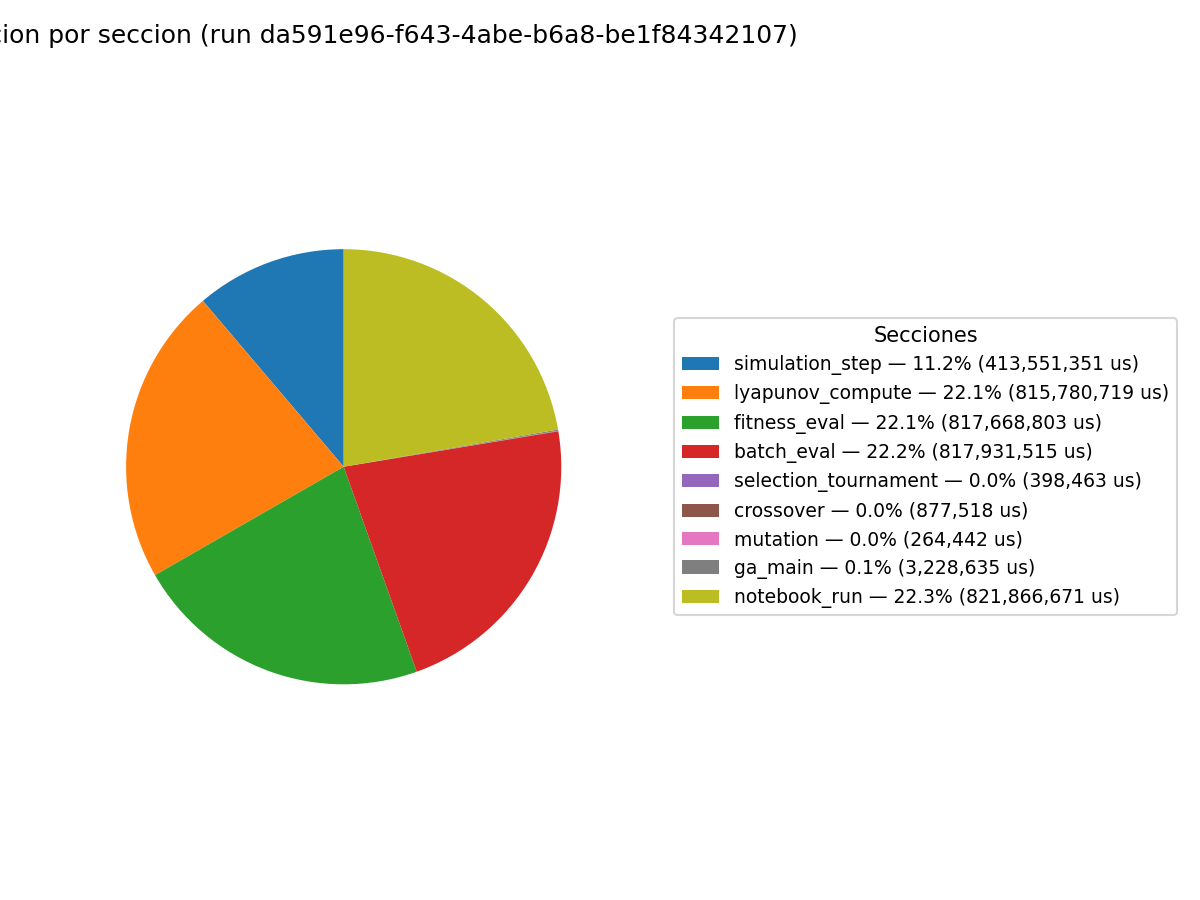
\includegraphics[width=0.85\textwidth]{img/resultados/caso03-metricasTiempo.png}
\caption{Resumen visual del CSV de timings.}
\label{fig:c01_timings} %chktex 24 %chktex 24
\end{figure}

\paragraph{D. Resultados y artefactos}
\begin{itemize}
    \item Diccionario \texttt{results} con masas óptimas, fitness y $\lambda$ final.
    \item Series \texttt{metrics.best\_lambda\_per\_epoch} y \texttt{metrics.best\_fitness\_per\_epoch} para análisis de convergencia.
    \item Trayectorias \texttt{traj\_original}, \texttt{traj\_opt} y \texttt{xyz\_tracks} listas para visualización.
    \item Animaciones MP4 generadas en \texttt{artifacts/caso03} y reportes de timings en \texttt{reports/}.
\end{itemize}

\paragraph{E. Conclusiones del caso}
\begin{itemize}
    \item El adaptador con impulsos periódicos permite estudiar de forma controlada las oscilaciones inducidas por “kicks” tangenciales.
    \item La solución óptima reduce el exponente de Lyapunov frente al estado base, indicando mayor estabilidad pese a los impulsos.
    \item Las animaciones 2D/3D muestran cómo el planeta mantiene órbitas cuasi periódicas tras los ajustes del algoritmo.
    \item Las estadísticas de timings identifican las secciones más costosas (evaluación larga, integración con impulsos), facilitando optimizaciones futuras.
\end{itemize}
